\documentclass[a4paper,10pt]{report}

\topmargin -2cm
%\topskip0cm
%\footskip0cm
%\headsep0cm
\parindent0cm
\oddsidemargin -1cm
\evensidemargin -1cm
\headheight 2cm
\textheight 24cm
\textwidth 18cm

\author{Daniel W\"aber (4049590)}
\title{\"Ubung}

\usepackage{ucs}
\usepackage[utf8x]{inputenc}
\usepackage{german}
\usepackage{color}
\usepackage{url}
\usepackage{graphicx}
\usepackage{algorithmic}

\pagestyle{empty}
\usepackage{makeidx}
\usepackage{amsmath}
\usepackage{amsfonts}
\usepackage{amssymb,euscript}
\usepackage{dsfont}
\usepackage{listings}
\usepackage{enumerate}
\newfont{\Fr}{eufm10}
\newfont{\Sc}{eusm10}
\newfont{\Bb}{msbm10}
\newcommand{\limin}{\lim_{n\rightarrow\infty}}
\newcommand{\limix}{\lim_{x\rightarrow\infty}}
\newcommand{\limun}{\lim_{n\rightarrow -\infty}}
\newcommand{\limux}{\lim_{n\rightarrow -\infty}}
\newcommand{\limx}{\lim_{x\rightarrow x_0}}
\newcommand{\limh}{\lim_{h\rightarrow 0}}
\newcommand{\defi}{\paragraph{Definition:}}
\newcommand{\bew}{\paragraph{Beweis:}}
\newcommand{\satz}{\paragraph{Satz:}}
\newcommand{\bsp}{\paragraph{Beispiel:}}
\newcommand{\lemma}{\paragraph{Lemma:}}
\newcommand{\N}{\mathds{N}}
\newcommand{\F}{\mathds{F}}
\newcommand{\Z}{\mathds{Z}}
\newcommand{\Q}{\mathds{Q}}
\newcommand{\R}{\mathds{R}}
\newcommand{\G}{\mathds{G}}
\newcommand{\C}{\mathds{C}}
\newcommand{\K}{\mathds{K}}
\newcommand{\A}{\mathds{A}}
\newcommand{\E}{\mathcal{E}}
\renewcommand{\P}{\mathcal{P}}
\newcommand{\sigA}{$\sigma$-Algebra }
\newcommand{\qed}{$\hfill\blacksquare$}
\newcommand{\arsinh}{\operatorname{arsinh} }
\newcommand{\arcosh}{\operatorname{arcosh} }
\newcommand{\gdw}{ $ \Leftrightarrow $ }
\newcommand{\tf}{ $ \Rightarrow $ }
\newcommand{\mgdw}{\Leftrightarrow}
\newcommand{\mtf}{\Rightarrow}
\newcommand{\Bild}{\text{Bild}}
\newcommand{\Kern}{\text{kern}}
\newcommand{\rg}{\text{rg}}
\newcommand{\deff}{\text{deff}}

\newcommand{\alphato}{\underset{\alpha}\to}
\newcommand{\betato}{\underset{\beta}\to}
\newcommand{\etato}{\underset{\eta}\to}
\newcommand{\ito}{\underset{i}\to}
\newcommand{\sto}{\underset{s}\to}
\newcommand{\kto}{\underset{k}\to}
\newcommand{\xto}{\underset{x}\to}

\usepackage{fancyhdr}
\pagestyle{fancy}
\lhead{Daniel Waeber\\Alex Muenn}
\chead{"Ubungsblatt \nr\\\today}
\rhead{Bildverarbeitung}


\newcommand{\nr}{2}
\lstset{language=matlab}

\begin{document}
\section*{Aufgabe 1 - FFT}
Die FFT implementierten wir nach dem in der Vorlesung vorgetellten Verfahren,
bei dem eine Umverteilung der Spalten der Fourier-Matrix angenommen wird und
damit auch die Zeilen des zu transformierenden Vektors/Matrix angepasst werden
m\"ussen. (Anmerkung: fft(x) arbeitet zeilenweise/auf einen Zeilenvektor)\\

\lstinputlisting[caption=func/fft.m,language=matlab]{func/fft.m}
Die \"aquivalente IFFT haben wir in der fftc.m implementiert, wobei der
unterschied in der Konjugation der Einheitswurzel besteht: 
$e^{-2\frac{\pi*i}{N}} \Leftrightarrow e^{2\frac{\pi*i}{N}} $

Im 2D sieht die Anwendung wie folgt aus: 
\begin{enumerate}
\item FFT auf Matrix anwenden, erhalten nach Zeilen Transformierte
\item Transformierte transponieren
\item FFT wieder auf Zeilen anwenden
\item Ergenis transponieren, weil \ldots
\end{enumerate}
\lstinputlisting[caption=FFT-2D,language=matlab]{func/fft2d.m}

\begin{figure}[H]
\begin{center}
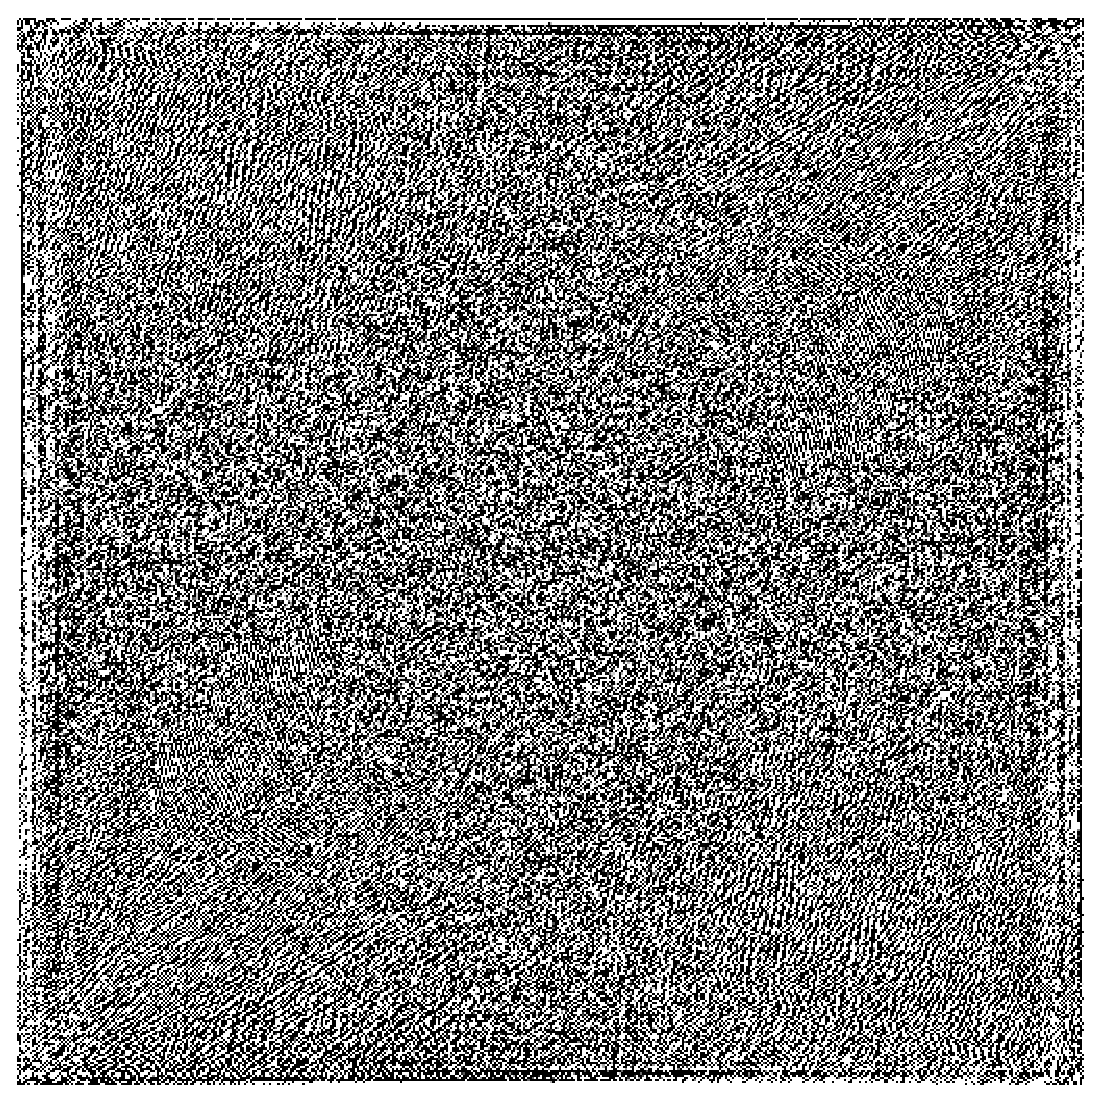
\includegraphics[width=50mm]{u02/f_out.eps}
\end{center}
\caption{Ergebnis: Lenna im Frequenzraum}
\end{figure}

\section*{Aufgabe 2 - Konvolution - DFT vs. FFT} 

Wie in der Vorlesung vorgestellt, wird die zur Faltung der Convulutionssatz verwendet.
Als Test-Kern haben wir ein einfach Glaettung angewandt:
\lstset{language=matlab}
\begin{lstlisting}[]
k = [0.4,0.2,0.1,zeros(1,n-5),0.1,0.2];
K = k' * k;
\end{lstlisting}

\begin{figure}[H]
\begin{center}
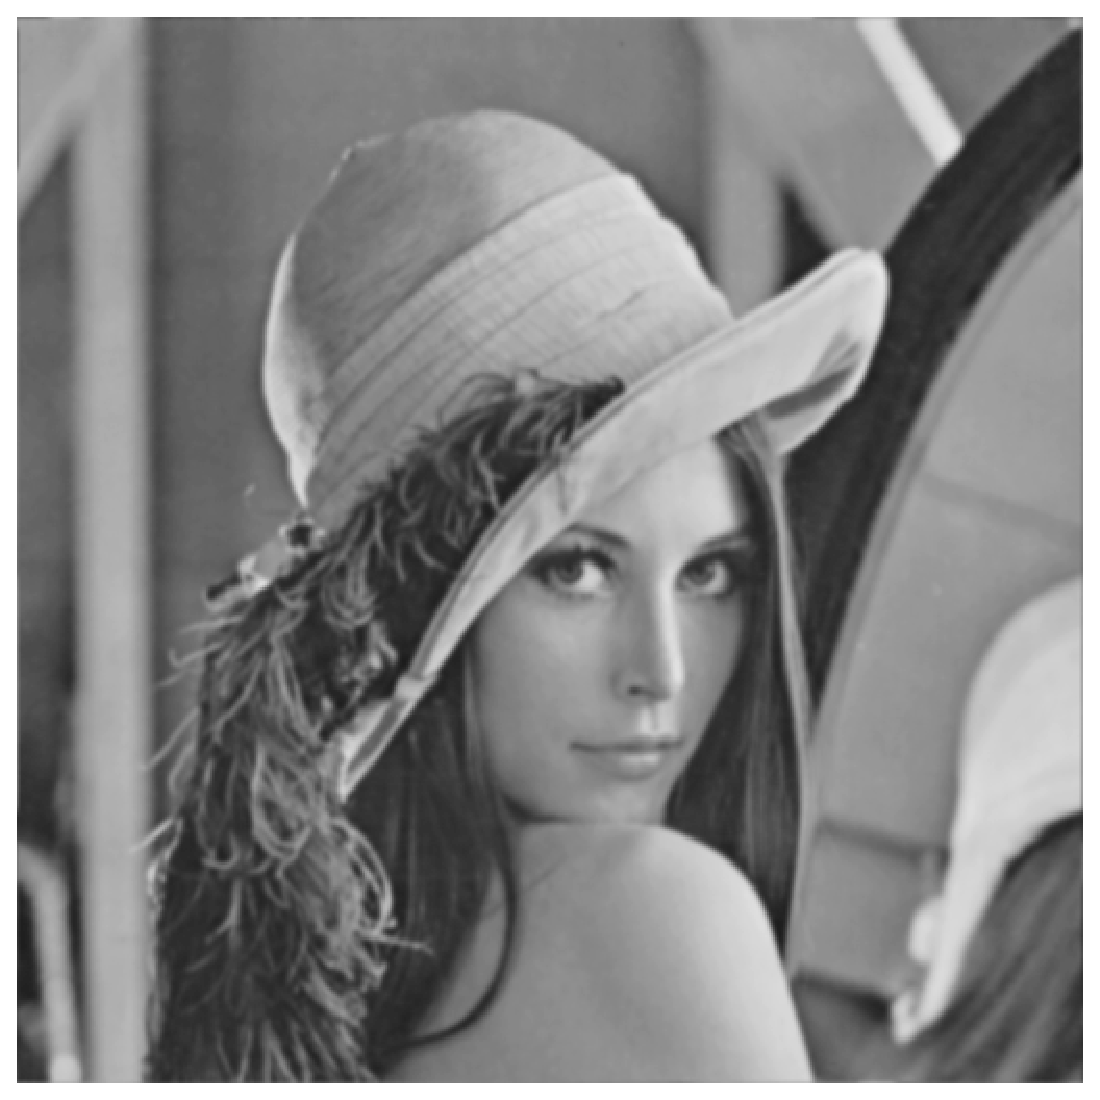
\includegraphics[width=50mm]{u02/c_out.eps}
\end{center}
\caption{Ergebnis: Glaettung}
\end{figure}

Schon bei der geringen Groesse des Bildes (512$\times$512) ist ein deutlicher
unterschied zwischen FFT und primitiver FT feststellbar.
\begin{verbatim}
using fft
Elapsed time is 4.93589 seconds.
using dft
Elapsed time is 18.4002 seconds.
\end{verbatim}

\end{document}
